%% Standalone lecture -- build with:  pdflatex -shell-escape experimentalDesign
%% Shared preamble for standalone lecture files.
%%
%% Every lecture begins with %% Shared preamble for standalone lecture files.
%%
%% Every lecture begins with %% Shared preamble for standalone lecture files.
%%
%% Every lecture begins with \input{preamble} and is compiled on its own:
%%     pdflatex -shell-escape <lecture>
%% There is no master lectures.tex any more -- the list of lectures lives in
%% lectures.yaml and is read by the build scripts.

\documentclass[25pt,landscape,footrule]{foils}
\input{macros_gen}
\backgroundsetup{contents={}}

\usepackage{stmaryrd}
\usepackage{ifthen}
\usepackage{pdf14}

% figures/ is not duplicated here -- the originals in ../lectures/figures are used
\graphicspath{{figures/}{../lectures/figures/}{~/Documents/figures/}{~/Documents/teaching/courses/comp6208/old_lectures/figures/}{~/Documents/teaching/courses/comp3008/new_lectures/figures/}{~/Documents/teaching/courses/comp6208/new_lectures/figures/}{~/Documents/teaching/courses/MLshort/figures/}{~/Documents/teaching/courses/comp3212/lectures/figures/}{/Users/apb1/Documents/teaching/courses/comp6208/github/lectures/figures}}

\date{}

\newcounter{lessoncnt}
\newcommand{\lesson}[1]{\setcounter{page}{1}%
\section{Mathematics of Machine Learning\\%
\vfill
\textcolor{red}{\textit{#1}}
\vfill}}
 and is compiled on its own:
%%     pdflatex -shell-escape <lecture>
%% There is no master lectures.tex any more -- the list of lectures lives in
%% lectures.yaml and is read by the build scripts.

\documentclass[25pt,landscape,footrule]{foils}
\input{macros_gen}
\backgroundsetup{contents={}}

\usepackage{stmaryrd}
\usepackage{ifthen}
\usepackage{pdf14}

% figures/ is not duplicated here -- the originals in ../lectures/figures are used
\graphicspath{{figures/}{../lectures/figures/}{~/Documents/figures/}{~/Documents/teaching/courses/comp6208/old_lectures/figures/}{~/Documents/teaching/courses/comp3008/new_lectures/figures/}{~/Documents/teaching/courses/comp6208/new_lectures/figures/}{~/Documents/teaching/courses/MLshort/figures/}{~/Documents/teaching/courses/comp3212/lectures/figures/}{/Users/apb1/Documents/teaching/courses/comp6208/github/lectures/figures}}

\date{}

\newcounter{lessoncnt}
\newcommand{\lesson}[1]{\setcounter{page}{1}%
\section{Mathematics of Machine Learning\\%
\vfill
\textcolor{red}{\textit{#1}}
\vfill}}
 and is compiled on its own:
%%     pdflatex -shell-escape <lecture>
%% There is no master lectures.tex any more -- the list of lectures lives in
%% lectures.yaml and is read by the build scripts.

\documentclass[25pt,landscape,footrule]{foils}
\input{macros_gen}
\backgroundsetup{contents={}}

\usepackage{stmaryrd}
\usepackage{ifthen}
\usepackage{pdf14}

% figures/ is not duplicated here -- the originals in ../lectures/figures are used
\graphicspath{{figures/}{../lectures/figures/}{~/Documents/figures/}{~/Documents/teaching/courses/comp6208/old_lectures/figures/}{~/Documents/teaching/courses/comp3008/new_lectures/figures/}{~/Documents/teaching/courses/comp6208/new_lectures/figures/}{~/Documents/teaching/courses/MLshort/figures/}{~/Documents/teaching/courses/comp3212/lectures/figures/}{/Users/apb1/Documents/teaching/courses/comp6208/github/lectures/figures}}

\date{}

\newcounter{lessoncnt}
\newcommand{\lesson}[1]{\setcounter{page}{1}%
\section{Mathematics of Machine Learning\\%
\vfill
\textcolor{red}{\textit{#1}}
\vfill}}


\begin{document}

\lesson{On Becoming a Scientist}
\vspace{-1cm}
\begin{center}
\noindent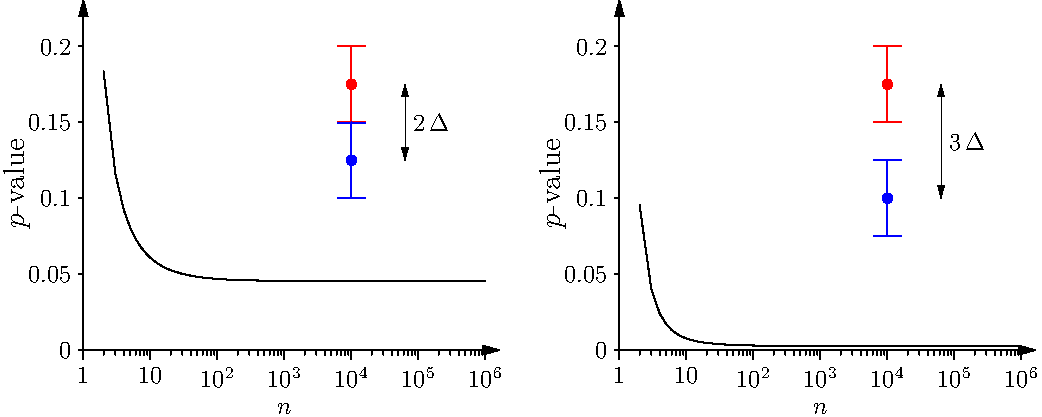
\includegraphics[height=100mm]{errorbarsT}
\end{center}
\keywords{interpeting data, standard errors, confidence tests}
%%%%%%%%%%%%%%%%%%%%%%% Next Slide %%%%%%%%%%%%%%%%%%%%%%%
\renewcommand{\Outline}{%
\begin{slide}
\section[1]{Outline}

\begin{minipage}{12cm}\raggedright
  \begin{enumerate}\squeeze
    \outlineitem{Outline}{outline}
    \outlineitem{Experimental Error}{errors}
    \outlineitem{Confidence Estimates}{confidence}
  \end{enumerate}
\end{minipage}\hfill
\begin{minipage}{10cm}
  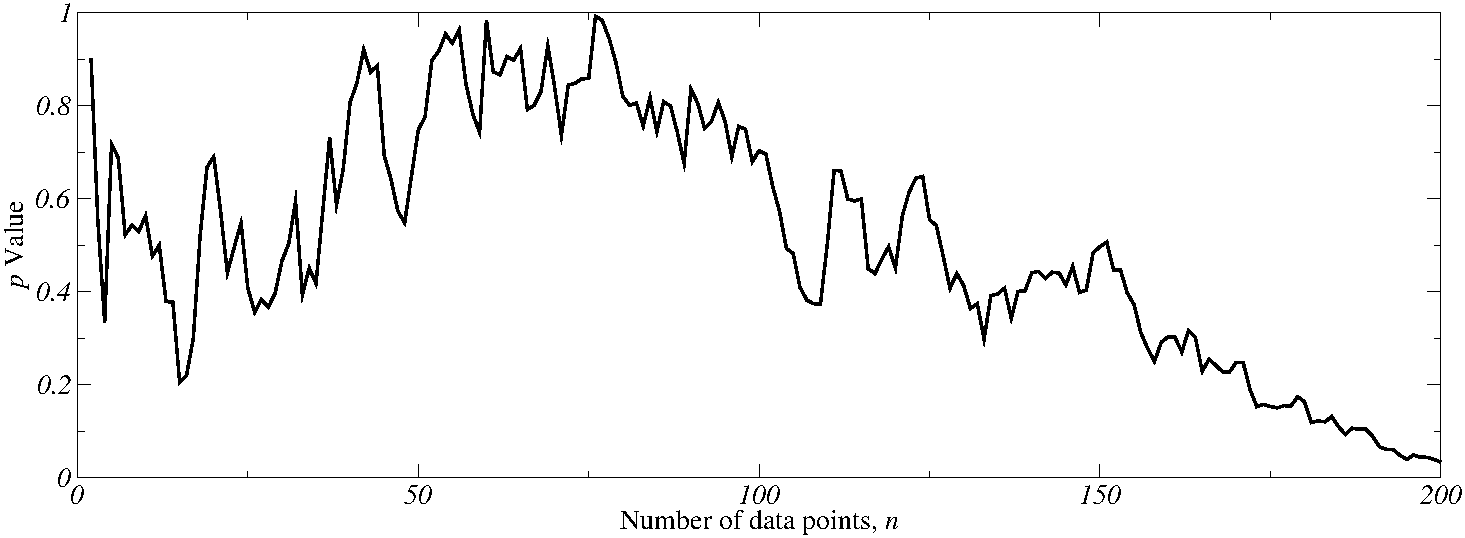
\includegraphics[width=10cm]{tTest}
\end{minipage}
\end{slide}
\addtocounter{outlineitem}{1}
}

\setcounter{outlineitem}{1}


%%%%%%%%%%%%%%%%%%%%%%% Next Slide %%%%%%%%%%%%%%%%%%%%%%%
\Outline % Outline
\toptarget{firstoutline}
%%%%%%%%%%%%%%%%%%%%%%% Next Slide %%%%%%%%%%%%%%%%%%%%%%%

\begin{slide}
\section{Experiments and Reproducibility}

\begin{PauseHighLight}
  \begin{itemize}
  \item One of the fundamental requirements of science is that
    experiments can be reproduced\pause
  \item This applies to machine learning and deep-learning as it does
    to particle physics, molecular biology, etc.\pause
  \item We need to describe completely what procedures were carried
    out\pause
  \item However, experiments have natural variability so what do we
    mean by repeatability?\pause
  \end{itemize}
\end{PauseHighLight}

\end{slide}

%%%%%%%%%%%%%%%%%%%%%%% Next Slide %%%%%%%%%%%%%%%%%%%%%%%

\begin{slide}
\section{Describing Research}

\begin{PauseHighLight}
  \begin{itemize}
  \item When describing research you need to find a story
    (narrative)\pause---why is the work you are doing
    interesting\pauseb
  \item You need to give a general motivation as well as a more
    detailed explanation of what you are specifically going to
    test\pause
  \item You then need to give enough details that someone can take
    your report/paper and reproduce what you are doing\pause
  \item These days it is also common practice to put the model you
    are using on-line\pause---but you should still describe everything
    in your report\pauseb
  \end{itemize}
\end{PauseHighLight}

\end{slide}

%%%%%%%%%%%%%%%%%%%%%%% Next Slide %%%%%%%%%%%%%%%%%%%%%%%

\begin{slide}
\section[-1]{Describing Your Experiments}

\begin{PauseHighLight}
  \begin{itemize}
  \item You need to tell the reader
    \begin{itemize}\squeeze
    \item What  your deep-learning architecture looks like\pause
    \item Your training set\pause
    \item How you partitioned your training set into train, validation
      and test sets\pause
    \item  Any preprocessing you performed\pause
    \item The optimiser you used, mini-batch size, learning rate\pause
    \item The number of epochs you trained for\pause
    \item Any hyper-parameter tuning you carried out\pause
    \item How long it took in clock time on the platform you are using\pause
    \end{itemize}
  \item You can put some of this into an appendix if necessary\pause
  \end{itemize}
\end{PauseHighLight}

\end{slide}

%%%%%%%%%%%%%%%%%%%%%%% Next Slide %%%%%%%%%%%%%%%%%%%%%%%

\begin{slide}
\section{Results}

\begin{PauseHighLight}
  \begin{itemize}
  \item A paper builds a story (thesis) based on experimental
    evidences\pause
  \item It is not enough to present results, it is also your job to
    interpret the results\pause
  \item Your results provide evidence in support of your thesis\pause
  \item But results all come with uncertainty.  If you tested on a
    different test set, or used a different training set then the
    answer would be different\pause
  \item \emph{Results are meaningless unless the uncertainty is quantified!}\pause
  \end{itemize}
\end{PauseHighLight}

\end{slide}

%%%%%%%%%%%%%%%%%%%%%%% Next Slide %%%%%%%%%%%%%%%%%%%%%%%
\Outline % Experimental Error
%%%%%%%%%%%%%%%%%%%%%%% Next Slide %%%%%%%%%%%%%%%%%%%%%%%

\begin{slide}
\section{Experimental Error}

\begin{PauseHighLight}
  \begin{itemize}
  \item Any empirical result is useless without some estimate of
    error\pause
  \item If you tell me algorithm A has a performance of 95\% and
    algorithm B has a performance of 97\%, how do I know that this
    didn't happen by chance?\pause
  \item Maybe algorithm A is actually better, but you got lucky (or
    unlucky)\pause
  \item We need to get a handle on the estimated experimental error\pause
  \end{itemize}
\end{PauseHighLight}

\end{slide}

%%%%%%%%%%%%%%%%%%%%%%% Next Slide %%%%%%%%%%%%%%%%%%%%%%%

\begin{slide}
\section{Datasets}

\begin{PauseHighLight}
  \begin{itemize}
  \item We assume that our test set consists of typical examples that
    we might encounter and that they are independent (e.g. we are not
    seeing the same example over and over again)\pause
  \item These are assumptions that are not always true\pause
  \item We need to think about it and if they are not true you may need
    to collect new data or be very cautious of the claims that you are
    making\pause
  \item However, if the person curating the training set did a good
    job then usually these are reasonable assumptions\pause
  \end{itemize}
\end{PauseHighLight}

\end{slide}

%%%%%%%%%%%%%%%%%%%%%%% Next Slide %%%%%%%%%%%%%%%%%%%%%%%

\begin{slide}
\section{Collecting Statistics}

\begin{PauseHighLight}
  \begin{itemize}
  \item Given some experimental measurements $\{X_i| i=1,2,\ldots,n\}$
    we can estimate the mean and variance
    \begin{align*}
      \hat{\mu}_n &= \frac{1}{n} \sum_{i=1}^n X_i &
      \hat{\sigma}_n^2 &= \frac{1}{n-1} \sum_{i=1}^n (X_i-\hat{\mu}_n)^2\pause
    \end{align*}
  \item These are not the true mean, $\mu=\av{X_i}$, and true variance
    $\sigma^2=\av{(X_i-\mu)^2}$, but they are unbiased estimates in that
    \begin{align*}
      \av{\hat{\mu}_n} &= \mu & \av{\hat{\sigma}_n^2} &= \sigma^2\pause
    \end{align*}
  \end{itemize}
\end{PauseHighLight}

\end{slide}

%%%%%%%%%%%%%%%%%%%%%%% Next Slide %%%%%%%%%%%%%%%%%%%%%%%

\begin{slide}
\section[-2]{Variance in Mean Estimator}

\begin{PauseHighLight}
  \begin{itemize}\small
    \item Consider the  mean squared error (MSE) of the estimator $\hat{\mu}_n$
      \begin{align*}
        \av{ (\hat{\mu}_n-\mu)^2 } &= \av{ \bra{\bra{\frac{1}{n}\sum_{i=1}^n
        X_i} - \mu}^2}\pause
        = \, \av{ \left( \frac{1}{n} \sum_{i=1}^n (X_i -\mu)\right)^2}\pause\\
        &= \frac{1}{n^2} \, \av{ \left(\sum_{i=1}^n (X_i -\mu)\right)\left(\sum_{j=1}^n (X_j -\mu)\right)\pause}\\
        &=\frac{1}{n^2} \, \av{ \sum_{i=1}^n (X_i -\mu)^2
          + \sum_{i=1}^n\sum_{j=1\atop j\neq i}^n (X_i-\mu)\,(X_j-\mu)}\pause\\
        &= \frac{1}{n^2}\sum_{i=1}^n \left( \av{(X_i -\mu)^2}
          + \sum_{j=1\atop j\neq i}^n
          \av{X_i-\mu}\,\av{X_j-\mu} \right)\pause\\
        &=\frac{1}{n^2} \sum_{i=1}^n \sigma^2\pause = \frac{1}{n} \sigma^2
        \pause
    \end{align*}
  
  \end{itemize}
\end{PauseHighLight}

\end{slide}

%%%%%%%%%%%%%%%%%%%%%%% Next Slide %%%%%%%%%%%%%%%%%%%%%%%

\begin{slide}
\section[-2]{Estimated Error in the Mean}

\begin{PauseHighLight}
  \begin{itemize}
  \item The root mean squared error (RMSE) is equal to 
    \begin{align*}
      \sqrt{\av{ (\hat{\mu}_n-\mu)^2 }} = \frac{\sigma}{\sqrt{n}}\pause
    \end{align*}
  \item The \emph{estimated error in the mean} or \emph{standard
      error} is defined as $\Delta = \frac{\hat{\sigma}_n}{\sqrt{n}}$
    where $\hat{\sigma}_n$ is the empirical estimate of the standard
    deviation\pause
  \item Traditionally we would write an experimental result as
    $\hat{\mu}_n \pm \Delta$\pause
  \item Also we only quote $\hat{\mu}_n$ up to the number of
    significant figures consistent with $\Delta$\pause
  \item Not $1.6582356 \pm 0.122543$ but $1.7 \pm 0.1$\pauseb
  \end{itemize}
\end{PauseHighLight}

\end{slide}

%%%%%%%%%%%%%%%%%%%%%%% Next Slide %%%%%%%%%%%%%%%%%%%%%%%

\begin{slide}
\section[-1]{Repeated Bernoulli Trials}

\begin{PauseHighLight}
  \begin{itemize}
  \item Suppose we are measuring a binary outcome, success or failure\pause
  \item Assuming the trials are independent (so called Bernoulli
    trials) then the only unknown is the probability, $p$, of a success\pause
  \item If we make $n$ trials then probability of $k$ successes is
    given by the binomial distribution
    \begin{align*}
      \Prob{K=k} = \binom{k}{n} p^k\,(1-p)^{n-k}\pause
    \end{align*}
  \item The mean and variance of $K$ are
    \begin{align*}
      \av{K} &= n\,p & \av{(K-n\,p)^2} = n\,p\,(1-p)\pause
    \end{align*}
  \end{itemize}
\end{PauseHighLight}

\end{slide}

%%%%%%%%%%%%%%%%%%%%%%% Next Slide %%%%%%%%%%%%%%%%%%%%%%%

\begin{slide}
\section[-2]{Mean Squared Error}
  
\begin{PauseHighLight}
  \begin{itemize}
  \item For the case of $n$ Bernoulli trials we can estimate the mean
    success rate
    \begin{align*}
      \hat{p} = \frac{K}{n}\pause
    \end{align*}
  \item The mean squared error (MSE) in this estimate is
    \begin{align*}
      \av{(\hat{p}-p)^2} &= \av{\bra{\frac{K}{n}-p}^2} = \frac{1}{n^2}
                 \av{\bra{K-n\,p}^2} \pause\\
      &= \frac{1}{n^2}\,n\,p\,(1-p)\pause = \frac{p\,(1-p)}{n}\pause
    \end{align*}
  \end{itemize}
\end{PauseHighLight}

\end{slide}

%%%%%%%%%%%%%%%%%%%%%%% Next Slide %%%%%%%%%%%%%%%%%%%%%%%

\begin{slide}
\section[-2]{Standard Error for Bernoulli Trials}

\begin{PauseHighLight}
  \begin{itemize}
  \item The estimated error in the mean is given by the root mean
    squared error (RMSE) $\sqrt{\av{(\hat{p}-p)^2}} = \sqrt{\frac{p\,(1-p)}{n}}\pause$
  \item We don't know $p$, but we can use an estimate, $\hat{p}=\frac{K}{n}$
    \begin{align*}
      \Delta \approx \sqrt{\frac{\hat{p}\,(1-\hat{p})}{n}}\pause
    \end{align*}
  \item We can also use a worst-case bound (when $p=\frac{1}{2}$)
    \begin{align*}
      \Delta \approx \frac{1}{2\,\sqrt{n}}\pause
    \end{align*}
    This is pessimistic if $p$ is small, although the previous
    estimate is optimistic if $\hat{p}=0$\pause 
  \end{itemize}
\end{PauseHighLight}

\end{slide}


%%%%%%%%%%%%%%%%%%%%%%% Next Slide %%%%%%%%%%%%%%%%%%%%%%%

\begin{slide}
\section[-2]{Errorbars}

\begin{PauseHighLight}
  \begin{itemize}
  \item There are different conventions on errorbars\pause
  \item Traditionally errorbars show the estimated error in the mean
    (standard error, $\Delta = \hat{\sigma}_n/\sqrt{n}$)\pause
  \item This means that about 30\% of the time the true mean would be
    outside the errorbar\pause
  \item Some people use 95\% confident intervals as errorbars, saying
    95\% of the time the true mean lies within the
    errorbars\pause---this corresponds to errorbars showing twice the
    standard error\pauseb
  \item Some people show the standard deviation as errorbars\pause,
    this tells you nothing about the confidence of the point you
    plot\pauseb---in my opinion it is just wrong\pauseb
  \end{itemize}
\end{PauseHighLight}

\end{slide}

%%%%%%%%%%%%%%%%%%%%%%% Next Slide %%%%%%%%%%%%%%%%%%%%%%%

\begin{slide}
\section[-2]{Box Plots}

\begin{center}
  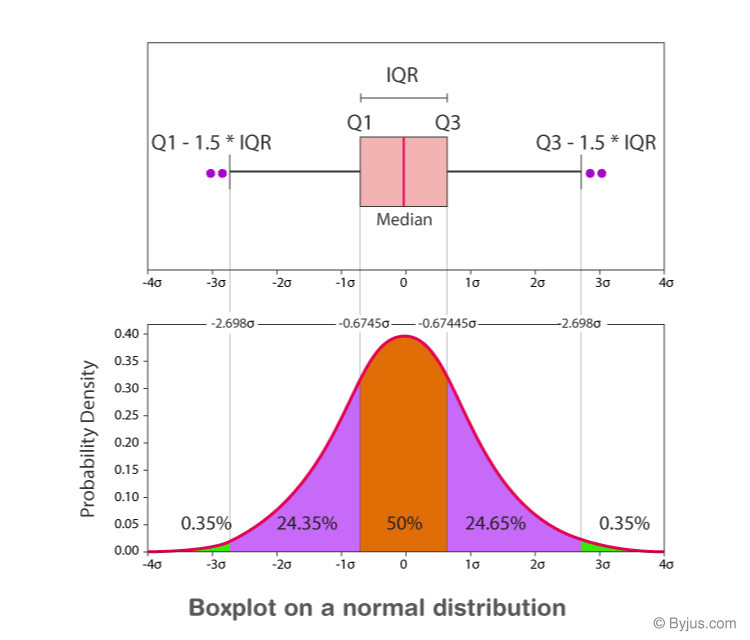
\includegraphics[width=0.8\linewidth]{boxPlot}
\end{center}

\end{slide}


%%%%%%%%%%%%%%%%%%%%%%% Next Slide %%%%%%%%%%%%%%%%%%%%%%%
\Outline % Confidence Measures
%%%%%%%%%%%%%%%%%%%%%%% Next Slide %%%%%%%%%%%%%%%%%%%%%%%

\begin{slide}
\section[-1]{Know What's Best}

\pb
\begin{itemize}
\item How do we know if model B is better than model A?\pauseh
\end{itemize}
\begin{center}
\multipdf[width=\textwidth]{simulation}\pause  
\end{center}
The more data we have the less likely we will make a mistake\pauseb
\end{slide}

%%%%%%%%%%%%%%%%%%%%%%% Next Slide %%%%%%%%%%%%%%%%%%%%%%%

\begin{slide}
\section{Quantifying Uncertainty}

\begin{PauseHighLight}
  \begin{itemize}
  \item We want a way of quantifying the chance that model B is better
    than model A\pause
  \item To do this we can consider a \emph{null hypothesis}
    \begin{center}
      \textit{We suppose that model $A$ and $B$ have the same performance}\pause
    \end{center}
  \item We then ask, under the null hypothesis, what is the chance of obtaining a gap in
    performance at least as big as the one we observed\pause
  \item This will depend on the number of observations and the
    empirical variance\pause
  \end{itemize}
\end{PauseHighLight}

\end{slide}

%%%%%%%%%%%%%%%%%%%%%%% Next Slide %%%%%%%%%%%%%%%%%%%%%%%

\begin{slide}
\section[-2]{T-tests}

\begin{PauseHighLight}
  \begin{itemize}
  \item The original t-test was invented by William Gosset who worked
    for the Guinness brewery in Dublin, but published under the
    pseudonym \textit{Student}\pause
  \item He worked with the null hypothesis that the distributions for A
    and B are normal with the same means and standard deviations\pause
  \item The slightly more common test is Welch's t-test where the null
    hypothesis is that the two datasets are normally distributed with
    the same means but different standard deviations\pause
  \item The gap is equal to the $t$ value
    \begin{align*}
      t = \frac{\hat{\mu}_A - \hat{\mu}_B}{\hat{\sigma}_{A,B}}\pause
    \end{align*}
  \end{itemize} 
\end{PauseHighLight}

\end{slide}

%%%%%%%%%%%%%%%%%%%%%%% Next Slide %%%%%%%%%%%%%%%%%%%%%%%

\begin{slide}
\section{Welch's T-Test}

\begin{PauseHighLight}
  \begin{itemize}
  \item For Welch's t-test
    \begin{align*}
      t &= \frac{\hat{\mu}_A - \hat{\mu}_B}{\hat{\sigma}_{A,B}}
      &
      \hat{\sigma}_{A,B} &= \sqrt{\frac{\hat{\sigma}_A^2}{n} +
        \frac{\hat{\sigma}_B^2}{m} }\pause 
    \end{align*}
  \item Where $p$ depends on $t$ and the \textit{number of degrees of
      freedom}
    \begin{align*}
      \nu = \frac{ \hat{\sigma}_{A,B}^2}{(\hat{\sigma}_A^2/n)^2/(n-1)
        + (\hat{\sigma}_B^2/m)^2/(m-1)}\pause
    \end{align*}
  \item The beauty of the $t$-test is that from $t$ and $\nu$ we can
    compute $p$\pause
  \item Small $p$ is good.  It shows the null hypothesis is unlikely\pause
  \end{itemize}
\end{PauseHighLight}

\end{slide}

%%%%%%%%%%%%%%%%%%%%%%% Next Slide %%%%%%%%%%%%%%%%%%%%%%%

\begin{slide}
\section{Statistical Significance}

\begin{PauseHighLight}
  \begin{itemize}
  \item It is common to say that $A$ is \textit{statistically significantly}
    better than $B$ if the probability of the observed $t$ value
    occurring given the null hypothesis is less than $0.05$\pause
  \item Statistically significant difference in performance does not
    mean that the difference is anything to care about\pause{} (that is
    a judgement call)\pauseb
  \item We are assuming the data is normally distributed\pause. We can
    check\pauseb, but no one does\pauseb. Usually its not a bad approximation
    if the data is not normal\pauseb, but there are exceptions\ldots\pauseb
  \end{itemize}
\end{PauseHighLight}

\end{slide}

%%%%%%%%%%%%%%%%%%%%%%% Next Slide %%%%%%%%%%%%%%%%%%%%%%%

\begin{slide}
\section[-2]{Example}

\begin{center}
  $X \sim \mathcal{N}(0.4, 1)$ \hfil $Y \sim \mathcal{N}(0.6, 0.25)$\\
  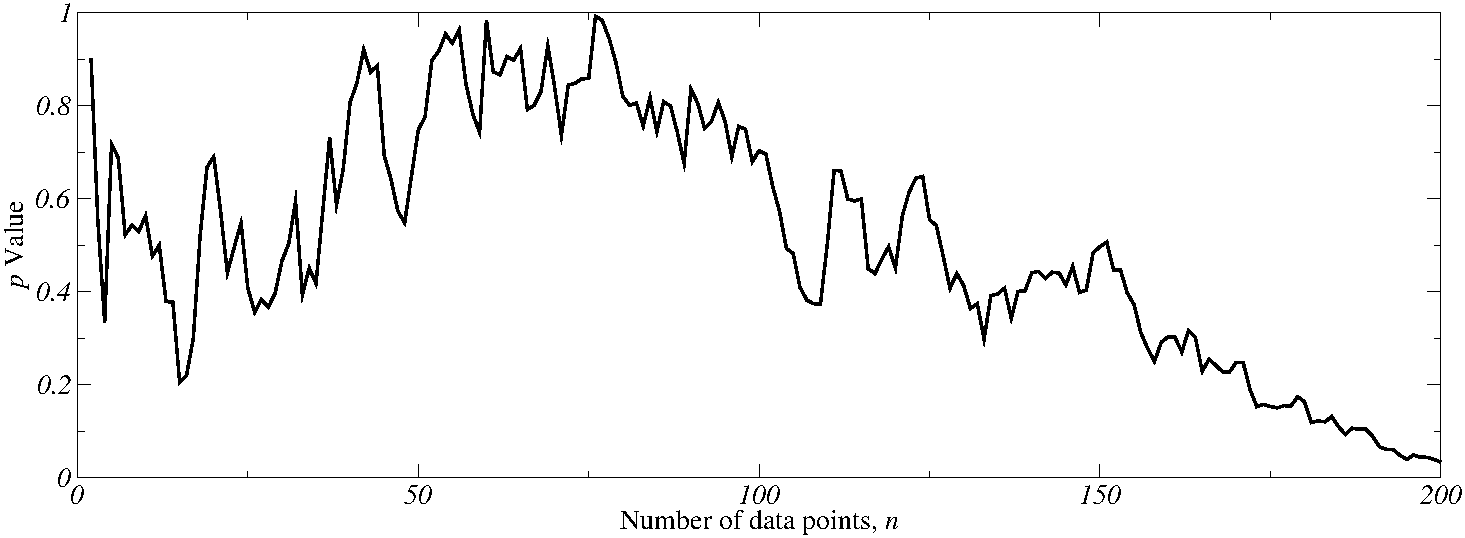
\includegraphics[width=0.8\linewidth]{tTest}\\
  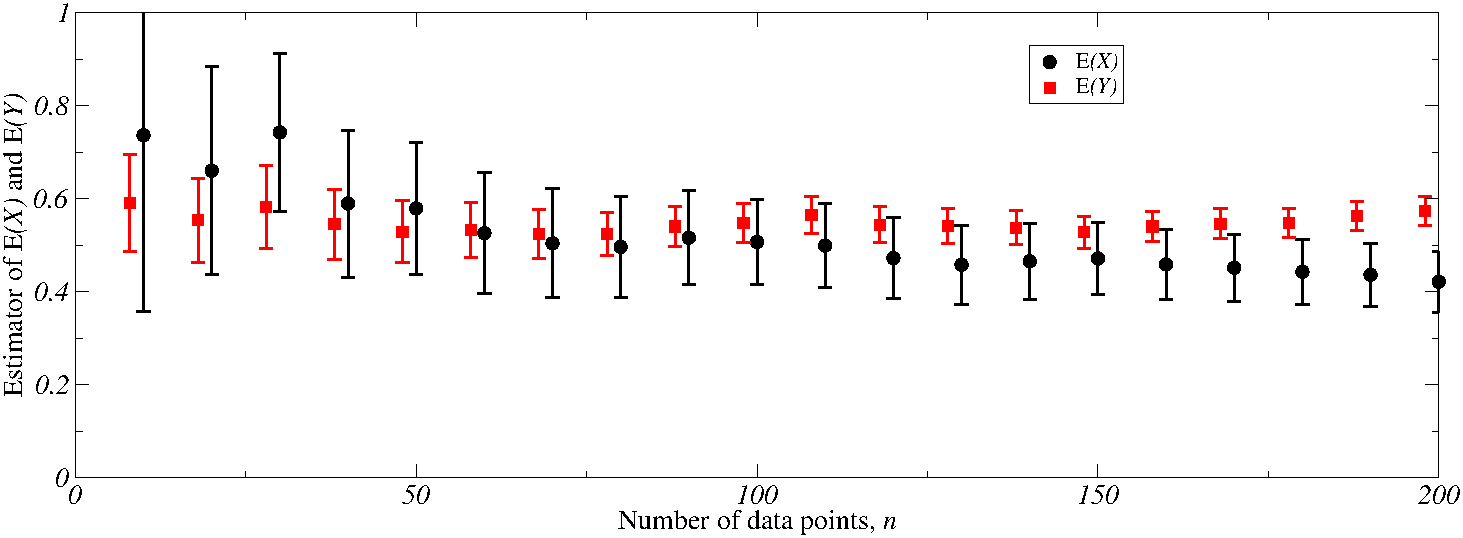
\includegraphics[width=0.8\linewidth]{tTesteb}
\end{center}

\end{slide}

%%%%%%%%%%%%%%%%%%%%%%% Next Slide %%%%%%%%%%%%%%%%%%%%%%%

\begin{slide}
\section{Error Bars and Significance}

\begin{center}
  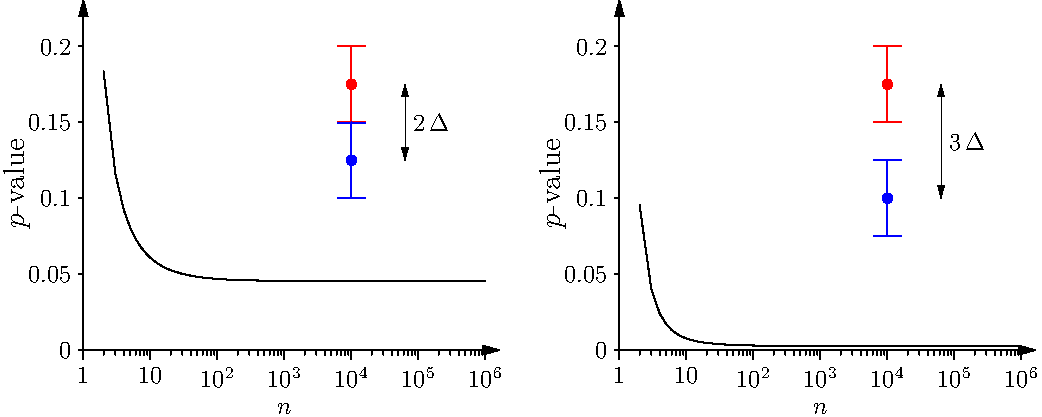
\includegraphics[width=\linewidth]{errorbarsT}\pause
\end{center}
\begin{PauseHighLight}
  \begin{itemize}
  \item If you have enough data points then when the errorbars (1
    standard error) are separate then the two distributions are
    significantly different\pause
  \end{itemize}
\end{PauseHighLight}

\end{slide}


%%%%%%%%%%%%%%%%%%%%%%% Next Slide %%%%%%%%%%%%%%%%%%%%%%%

\begin{slide}
\section[-1]{Paired T-Test}

\begin{PauseHighLight}
  \begin{itemize}
  \item Sometimes the fluctuations in performance will come both from
    the test example and from the difference in performance\pause
  \item For example model A might always be better than model B, but
    the performance fluctuates depending on the example\pause
  \item A normal t-test might not show any significant
    different\pause
  \item Using a paired t-test we instead use
    \begin{align*}
      \hat{\sigma}^2_{X+Y} &=
      \frac{\hat{\sigma}_X^2+\hat{\sigma}_Y^2-\hat{c}_{X,Y}}{n}
\\
      \hat{c}_{X,Y} &= \frac{1}{n-1} \sum_{i=1}^n
      (X_i-\hat{\mu}_X)\,(Y_i-\hat{\mu}_Y)\pause
    \end{align*}
  \end{itemize}
\end{PauseHighLight}

\end{slide}

%%%%%%%%%%%%%%%%%%%%%%% Next Slide %%%%%%%%%%%%%%%%%%%%%%%

\begin{slide}
\section[-2]{Paired T-Test Example}

\begin{center}
  $X \sim Z + X_1$ \hfil $Y \sim Z + Y_1$\\
  $Z \sim \mathcal{N}(0, 0.8)$ \hfil $X_1 \sim \mathcal{N}(0.4, 0.2)$ \hfil $Y_1 \sim \mathcal{N}(0.6, 0.2)$\\
  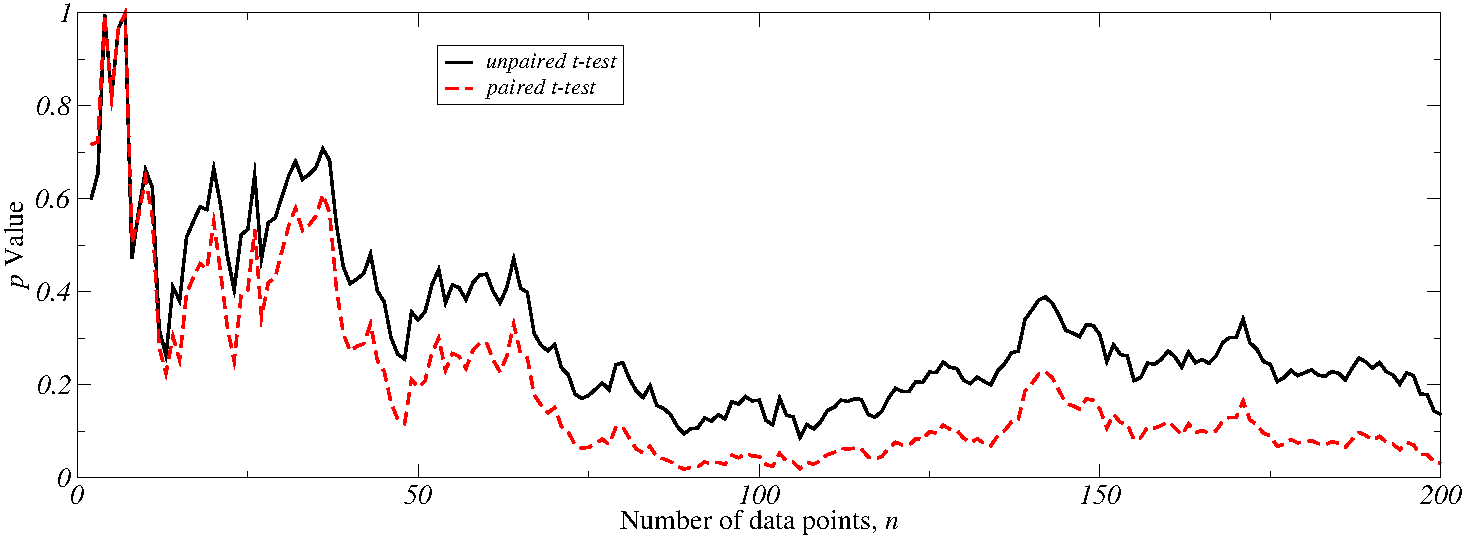
\includegraphics[width=0.8\linewidth]{pairedTtest}\\
  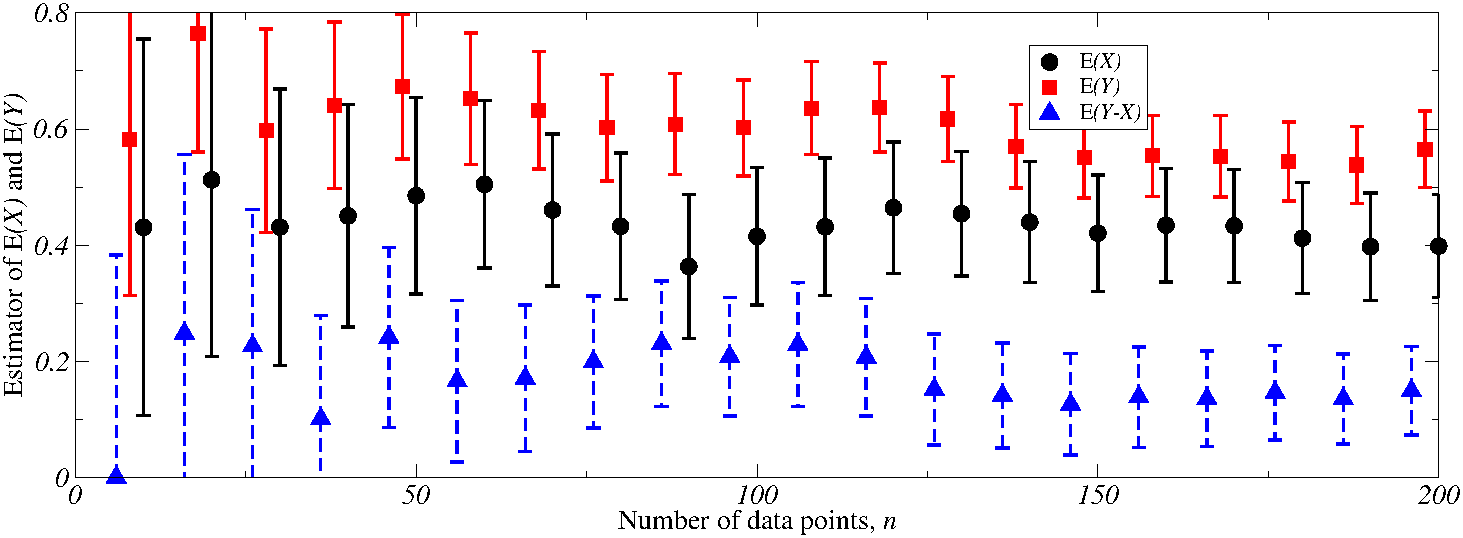
\includegraphics[width=0.8\linewidth]{pairedTtesteb}
\end{center}

\end{slide}

%%%%%%%%%%%%%%%%%%%%%%% Next Slide %%%%%%%%%%%%%%%%%%%%%%%

\begin{slide}
\section{Cheating Significant Tests}

\begin{PauseHighLight}
  \begin{itemize}
  \item You should only run your t-test once\pause
  \item If you run multiple t-tests until you get one with $p<0.05$
    then you have cheated\pause
  \item With a $p$ value of 0.05 you expect to find the observed $t$
    value given the null hypothesis once every 20 trials\pause---if
    you do the t-test twice you should expect this to happen every 10
    trials (i.e.{} $p=0.1$)\pauseb
  \item If you run $t$-tests until you find a $p$ value of 0.05 you
    are cheating\pause
  \item If you want to compare many different models then you should
    use ANOVA instead\pause
  \end{itemize}
\end{PauseHighLight}

\end{slide}



%%%%%%%%%%%%%%%%%%%%%%% Next Slide %%%%%%%%%%%%%%%%%%%%%%%

\begin{slide}
\section{Computing Significance Ab-Initio}

\begin{PauseHighLight}
  \begin{itemize}
  \item The $t$-test results follow from a beautiful, but
    difficult calculation\pause
  \item However, you can simulate the null-hypothesis multiple times
    and measure empirically the number of times the $t$-value exceeds
    the observed $t$-values\pause
  \item This isn't necessary under the assumptions that the data is
    normally distributed (done by Student and Welch)\pause
  \item However, there are other times where you want to show that
    what you have found has not happened by chance\pause.  Often it is
    easy to simulate a null hypothesis\pause
  \end{itemize}
\end{PauseHighLight}

\end{slide}

%%%%%%%%%%%%%%%%%%%%%%% Next Slide %%%%%%%%%%%%%%%%%%%%%%%

\begin{slide}
\section[-2]{Good, Bad and the Ugly}

\begin{PauseHighLight}
  \begin{itemize}
  \item What I've told you is true of data that follows well behaved
    distributions\pause
  \item Just occasionally you come across data that has long (thick)
    tails
    \vspace*{-5mm}
    \begin{center}
      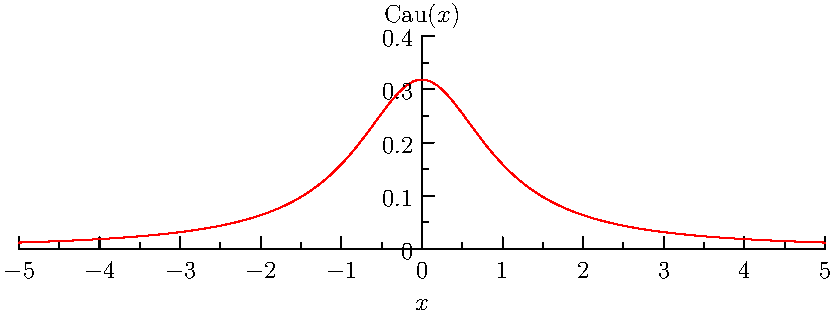
\includegraphics[width=0.7\linewidth]{cauchy}\pause
    \end{center}
    \vspace*{-5mm}
  \item Here taking the average of many samples might not give you
    reliable estimates of the mean\pause
  \item This isn't that common, but when nothing seems to make sense
    plot a histogram of the data and check for thick tails\pause
  \end{itemize}
\end{PauseHighLight}

\end{slide}

%%%%%%%%%%%%%%%%%%%%%%% Next Slide %%%%%%%%%%%%%%%%%%%%%%%

\begin{slide}
\section{Lessons}

\begin{PauseHighLight}
  \begin{itemize}
  \item You need to understand the errors in your data\pause
  \item Computing the standard error is always necessary\pause
  \item In some cases you can quantify your certainty that A is better
    than B using statistical confidence tests---t-tests\pause{} (other
    tests are available)\pauseb
  \item You need to apply common sense in interpreting data\pause
  \item \emph{The person you cheat when you don't do this is yourself}\pauseb
  \end{itemize}
\end{PauseHighLight}

\end{slide}


%%% Local Variables:
%%% TeX-master: "lectures"
%%% End:

\end{document}
